% Options for packages loaded elsewhere
\PassOptionsToPackage{unicode}{hyperref}
\PassOptionsToPackage{hyphens}{url}
%
\documentclass[
]{article}
\usepackage{amsmath,amssymb}
\usepackage{iftex}
\ifPDFTeX
  \usepackage[T1]{fontenc}
  \usepackage[utf8]{inputenc}
  \usepackage{textcomp} % provide euro and other symbols
\else % if luatex or xetex
  \usepackage{unicode-math} % this also loads fontspec
  \defaultfontfeatures{Scale=MatchLowercase}
  \defaultfontfeatures[\rmfamily]{Ligatures=TeX,Scale=1}
\fi
\usepackage{lmodern}
\ifPDFTeX\else
  % xetex/luatex font selection
\fi
% Use upquote if available, for straight quotes in verbatim environments
\IfFileExists{upquote.sty}{\usepackage{upquote}}{}
\IfFileExists{microtype.sty}{% use microtype if available
  \usepackage[]{microtype}
  \UseMicrotypeSet[protrusion]{basicmath} % disable protrusion for tt fonts
}{}
\makeatletter
\@ifundefined{KOMAClassName}{% if non-KOMA class
  \IfFileExists{parskip.sty}{%
    \usepackage{parskip}
  }{% else
    \setlength{\parindent}{0pt}
    \setlength{\parskip}{6pt plus 2pt minus 1pt}}
}{% if KOMA class
  \KOMAoptions{parskip=half}}
\makeatother
\usepackage{xcolor}
\usepackage[margin=1in]{geometry}
\usepackage{color}
\usepackage{fancyvrb}
\newcommand{\VerbBar}{|}
\newcommand{\VERB}{\Verb[commandchars=\\\{\}]}
\DefineVerbatimEnvironment{Highlighting}{Verbatim}{commandchars=\\\{\}}
% Add ',fontsize=\small' for more characters per line
\usepackage{framed}
\definecolor{shadecolor}{RGB}{248,248,248}
\newenvironment{Shaded}{\begin{snugshade}}{\end{snugshade}}
\newcommand{\AlertTok}[1]{\textcolor[rgb]{0.94,0.16,0.16}{#1}}
\newcommand{\AnnotationTok}[1]{\textcolor[rgb]{0.56,0.35,0.01}{\textbf{\textit{#1}}}}
\newcommand{\AttributeTok}[1]{\textcolor[rgb]{0.13,0.29,0.53}{#1}}
\newcommand{\BaseNTok}[1]{\textcolor[rgb]{0.00,0.00,0.81}{#1}}
\newcommand{\BuiltInTok}[1]{#1}
\newcommand{\CharTok}[1]{\textcolor[rgb]{0.31,0.60,0.02}{#1}}
\newcommand{\CommentTok}[1]{\textcolor[rgb]{0.56,0.35,0.01}{\textit{#1}}}
\newcommand{\CommentVarTok}[1]{\textcolor[rgb]{0.56,0.35,0.01}{\textbf{\textit{#1}}}}
\newcommand{\ConstantTok}[1]{\textcolor[rgb]{0.56,0.35,0.01}{#1}}
\newcommand{\ControlFlowTok}[1]{\textcolor[rgb]{0.13,0.29,0.53}{\textbf{#1}}}
\newcommand{\DataTypeTok}[1]{\textcolor[rgb]{0.13,0.29,0.53}{#1}}
\newcommand{\DecValTok}[1]{\textcolor[rgb]{0.00,0.00,0.81}{#1}}
\newcommand{\DocumentationTok}[1]{\textcolor[rgb]{0.56,0.35,0.01}{\textbf{\textit{#1}}}}
\newcommand{\ErrorTok}[1]{\textcolor[rgb]{0.64,0.00,0.00}{\textbf{#1}}}
\newcommand{\ExtensionTok}[1]{#1}
\newcommand{\FloatTok}[1]{\textcolor[rgb]{0.00,0.00,0.81}{#1}}
\newcommand{\FunctionTok}[1]{\textcolor[rgb]{0.13,0.29,0.53}{\textbf{#1}}}
\newcommand{\ImportTok}[1]{#1}
\newcommand{\InformationTok}[1]{\textcolor[rgb]{0.56,0.35,0.01}{\textbf{\textit{#1}}}}
\newcommand{\KeywordTok}[1]{\textcolor[rgb]{0.13,0.29,0.53}{\textbf{#1}}}
\newcommand{\NormalTok}[1]{#1}
\newcommand{\OperatorTok}[1]{\textcolor[rgb]{0.81,0.36,0.00}{\textbf{#1}}}
\newcommand{\OtherTok}[1]{\textcolor[rgb]{0.56,0.35,0.01}{#1}}
\newcommand{\PreprocessorTok}[1]{\textcolor[rgb]{0.56,0.35,0.01}{\textit{#1}}}
\newcommand{\RegionMarkerTok}[1]{#1}
\newcommand{\SpecialCharTok}[1]{\textcolor[rgb]{0.81,0.36,0.00}{\textbf{#1}}}
\newcommand{\SpecialStringTok}[1]{\textcolor[rgb]{0.31,0.60,0.02}{#1}}
\newcommand{\StringTok}[1]{\textcolor[rgb]{0.31,0.60,0.02}{#1}}
\newcommand{\VariableTok}[1]{\textcolor[rgb]{0.00,0.00,0.00}{#1}}
\newcommand{\VerbatimStringTok}[1]{\textcolor[rgb]{0.31,0.60,0.02}{#1}}
\newcommand{\WarningTok}[1]{\textcolor[rgb]{0.56,0.35,0.01}{\textbf{\textit{#1}}}}
\usepackage{longtable,booktabs,array}
\usepackage{calc} % for calculating minipage widths
% Correct order of tables after \paragraph or \subparagraph
\usepackage{etoolbox}
\makeatletter
\patchcmd\longtable{\par}{\if@noskipsec\mbox{}\fi\par}{}{}
\makeatother
% Allow footnotes in longtable head/foot
\IfFileExists{footnotehyper.sty}{\usepackage{footnotehyper}}{\usepackage{footnote}}
\makesavenoteenv{longtable}
\usepackage{graphicx}
\makeatletter
\def\maxwidth{\ifdim\Gin@nat@width>\linewidth\linewidth\else\Gin@nat@width\fi}
\def\maxheight{\ifdim\Gin@nat@height>\textheight\textheight\else\Gin@nat@height\fi}
\makeatother
% Scale images if necessary, so that they will not overflow the page
% margins by default, and it is still possible to overwrite the defaults
% using explicit options in \includegraphics[width, height, ...]{}
\setkeys{Gin}{width=\maxwidth,height=\maxheight,keepaspectratio}
% Set default figure placement to htbp
\makeatletter
\def\fps@figure{htbp}
\makeatother
\setlength{\emergencystretch}{3em} % prevent overfull lines
\providecommand{\tightlist}{%
  \setlength{\itemsep}{0pt}\setlength{\parskip}{0pt}}
\setcounter{secnumdepth}{-\maxdimen} % remove section numbering
\ifLuaTeX
  \usepackage{selnolig}  % disable illegal ligatures
\fi
\usepackage{bookmark}
\IfFileExists{xurl.sty}{\usepackage{xurl}}{} % add URL line breaks if available
\urlstyle{same}
\hypersetup{
  pdftitle={Tutorial},
  hidelinks,
  pdfcreator={LaTeX via pandoc}}

\title{Tutorial}
\author{}
\date{\vspace{-2.5em}}

\begin{document}
\maketitle

\begin{Shaded}
\begin{Highlighting}[]
\CommentTok{\#load Lund Taxonomy Classifier}
\FunctionTok{library}\NormalTok{(LundTax2023Classifier)}
\FunctionTok{library}\NormalTok{(knitr)}
\FunctionTok{library}\NormalTok{(grid)}
\end{Highlighting}
\end{Shaded}

\section{Lund Taxonomy Classifier}\label{lund-taxonomy-classifier}

This package depends on a set of internal and exported functions. The
main funcitons inteded for the user are; \texttt{lundtax\_predict\_sub},
\texttt{lundtax\_calc\_sigscore}, \texttt{plot\_hm\_signatures},
\texttt{plot\_hm\_sigscores}, \texttt{plot\_ranked\_score}. In this
tutorial, we will demonstrate how to use these functions, using the
bundled data to get the most out from this package.

\subsection{Bundled Data}\label{bundled-data}

Before we get started, let's start with exploring some of the relevant
bunlded data objects.

\subsubsection{Expression Data}\label{expression-data}

This package includes an example expression data set. This data is a
subset of samples from the Sjodahl 2017 paper. Let's first see the
dimensions of the data object.

\begin{Shaded}
\begin{Highlighting}[]
\FunctionTok{dim}\NormalTok{(sjodahl\_2017)}
\end{Highlighting}
\end{Shaded}

\begin{verbatim}
## [1] 15697   267
\end{verbatim}

The expression data set has 15607 rows (genes) and 267 columns
(samples). Let's have a look at the a the first 5 rows and 5 columns to
get an idea of what the data looks like.

\begin{Shaded}
\begin{Highlighting}[]
\NormalTok{knitr}\SpecialCharTok{::}\FunctionTok{kable}\NormalTok{(sjodahl\_2017[}\DecValTok{1}\SpecialCharTok{:}\DecValTok{5}\NormalTok{, }\DecValTok{1}\SpecialCharTok{:}\DecValTok{5}\NormalTok{], }
             \AttributeTok{caption =} \StringTok{"Table 1. Bundled expression data subset"}\NormalTok{)}
\end{Highlighting}
\end{Shaded}

\begin{longtable}[]{@{}lrrrrr@{}}
\caption{Table 1. Bundled expression data subset}\tabularnewline
\toprule\noalign{}
& 1.CEL & 2.CEL & 3.CEL & 4.CEL & 5.CEL \\
\midrule\noalign{}
\endfirsthead
\toprule\noalign{}
& 1.CEL & 2.CEL & 3.CEL & 4.CEL & 5.CEL \\
\midrule\noalign{}
\endhead
\bottomrule\noalign{}
\endlastfoot
A1CF & 4.248274 & 4.153923 & 4.186689 & 4.877813 & 4.106269 \\
A2M & 8.348800 & 7.969504 & 10.755738 & 8.467495 & 8.979223 \\
A2ML1 & 6.694896 & 4.442973 & 8.871067 & 4.392010 & 7.685045 \\
A4GALT & 7.255671 & 6.337239 & 6.925670 & 6.239185 & 6.032115 \\
A4GNT & 3.740418 & 3.830598 & 3.999331 & 3.813662 & 3.718752 \\
\end{longtable}

\subsubsection{Metadata}\label{metadata}

The package also includes meta data for the expression data. The
metadata can be used to aggregate the prediction calls, allowing for
interesting association between various metadata variables and specific
subtype. Let's explore this data set by overviewing what clinical
information is available.

\begin{Shaded}
\begin{Highlighting}[]
\FunctionTok{str}\NormalTok{(sjodahl\_2017\_meta)}
\end{Highlighting}
\end{Shaded}

\begin{verbatim}
## 'data.frame':    267 obs. of  25 variables:
##  $ sample_id        : chr  "1.CEL" "2.CEL" "3.CEL" "4.CEL" ...
##  $ cluster_order    : int  13 162 154 11 251 55 254 278 155 101 ...
##  $ age              : num  74.7 53.6 65.5 70.8 64.2 67.2 77.3 66.2 59.6 64.1 ...
##  $ gender           : Factor w/ 2 levels "Female","Male": 2 2 2 2 1 2 2 2 1 2 ...
##  $ region_cx        : Factor w/ 4 levels "HBG","LUND","MALMO",..: 3 3 3 3 3 3 3 3 1 3 ...
##  $ turb_grade       : Factor w/ 3 levels "0","1","N/A": 2 3 3 2 2 2 2 3 2 2 ...
##  $ turb_stage       : Factor w/ 3 levels "0","1","N/A": 2 2 2 2 2 2 2 1 2 2 ...
##  $ turb_skiv        : Factor w/ 3 levels "0","1","N/A": 1 1 1 2 2 1 2 1 2 1 ...
##  $ turb_cis         : Factor w/ 3 levels "0","1","N/A": 1 1 1 1 1 1 1 1 1 2 ...
##  $ turb_lvi         : Factor w/ 3 levels "0","1","N/A": 2 1 1 2 2 2 2 2 1 1 ...
##  $ turb_necros      : Factor w/ 4 levels "0","1","2","N/A": 1 1 2 2 3 3 3 3 2 2 ...
##  $ turb_apoptos     : Factor w/ 3 levels "0","1","N/A": 2 1 1 2 2 2 2 2 2 2 ...
##  $ variant_histology: Factor w/ 2 levels "0","1": 1 2 2 1 1 1 1 2 1 1 ...
##  $ cT               : Factor w/ 5 levels "1","2","3","4",..: 3 2 1 2 2 3 2 2 3 2 ...
##  $ cN               : Factor w/ 3 levels "0","1","N/A": 1 1 1 1 1 1 1 1 1 1 ...
##  $ hydroneph        : Factor w/ 2 levels "0","1": 2 1 1 1 1 1 2 1 1 2 ...
##  $ pTCx             : Factor w/ 10 levels "0","1","2","3",..: 6 8 5 8 4 5 1 2 8 9 ...
##  $ pN               : Factor w/ 5 levels "0","1","2","3",..: 3 1 1 1 1 1 3 1 1 3 ...
##  $ adj_chemo        : Factor w/ 2 levels "0","1": 2 1 1 1 1 1 1 1 1 2 ...
##  $ surv_os_event    : Factor w/ 2 levels "0","1": 2 2 1 2 1 2 2 2 2 2 ...
##  $ surv_os_time     : num  12.8 13.5 100.4 3 77.6 ...
##  $ surv_css_event   : Factor w/ 2 levels "0","1": 2 2 1 1 1 2 2 1 1 2 ...
##  $ surv_css_time    : num  12.8 13.5 100.4 3 77.6 ...
##  $ surv_pfs_event   : Factor w/ 2 levels "0","1": 2 2 1 1 1 2 2 1 1 2 ...
##  $ surv_pfs_time    : num  11.6 10.6 100.4 3 77.6 ...
\end{verbatim}

If the user wants to use their own metadata, this should be in a data
frame format wiith unique sample identifiers in a column called
\texttt{sample\_id}. For a more detailed explanation of the variables,
see that data set documentation.

\subsubsection{Other Bundled Objects}\label{other-bundled-objects}

this package also includes a variety of data objects needed for the
predictor. For example, classifiers for predicting grade and subtype,
lists with genes identifiers for making prediction calls and gene
signatures. Let's explore a few of these.

The \texttt{gene\_list} holds information on gene identifiers that the
predictor is based on. This object has gene identfiers in both HGNC and
Ensembl format, allowing the incoming data to be in either of these
formats.

\begin{Shaded}
\begin{Highlighting}[]
\NormalTok{knitr}\SpecialCharTok{::}\FunctionTok{kable}\NormalTok{(}\FunctionTok{head}\NormalTok{(gene\_list, }\DecValTok{5}\NormalTok{),}
             \AttributeTok{caption =} \StringTok{"Table 2. Gene List"}\NormalTok{)}
\end{Highlighting}
\end{Shaded}

\begin{longtable}[]{@{}ll@{}}
\caption{Table 2. Gene List}\tabularnewline
\toprule\noalign{}
ensembl\_gene\_id & hgnc\_symbol \\
\midrule\noalign{}
\endfirsthead
\toprule\noalign{}
ensembl\_gene\_id & hgnc\_symbol \\
\midrule\noalign{}
\endhead
\bottomrule\noalign{}
\endlastfoot
ENSG00000109576 & AADAT \\
ENSG00000183044 & ABAT \\
ENSG00000108846 & ABCC3 \\
ENSG00000114770 & ABCC5 \\
ENSG00000106077 & ABHD11 \\
\end{longtable}

How many genes in total, are included in the \texttt{gene\_list} object?

\begin{Shaded}
\begin{Highlighting}[]
\FunctionTok{nrow}\NormalTok{(gene\_list)}
\end{Highlighting}
\end{Shaded}

\begin{verbatim}
## [1] 1900
\end{verbatim}

The \texttt{signatures} object has all the information on what genes are
associated with what signature. This object is a list of 6 data frames,
for different signatures. Typically, the columns of each data frame are
the following; \texttt{hgnc\_symbol}, \texttt{ensembl\_gene\_id} and
\texttt{signature}. Let's have a look at the immune signatures object in
this list.

\begin{Shaded}
\begin{Highlighting}[]
\NormalTok{knitr}\SpecialCharTok{::}\FunctionTok{kable}\NormalTok{(}\FunctionTok{table}\NormalTok{(signatures}\SpecialCharTok{$}\NormalTok{immune}\SpecialCharTok{$}\NormalTok{signature), }
             \AttributeTok{caption =} \StringTok{"Table 3. Immune Signatures"}\NormalTok{, }
             \AttributeTok{col.names =} \FunctionTok{c}\NormalTok{(}\StringTok{"Signature"}\NormalTok{, }\StringTok{"Genes (n)"}\NormalTok{))}
\end{Highlighting}
\end{Shaded}

\begin{longtable}[]{@{}lr@{}}
\caption{Table 3. Immune Signatures}\tabularnewline
\toprule\noalign{}
Signature & Genes (n) \\
\midrule\noalign{}
\endfirsthead
\toprule\noalign{}
Signature & Genes (n) \\
\midrule\noalign{}
\endhead
\bottomrule\noalign{}
\endlastfoot
B-cells & 8 \\
Cytotoxicity Score & 10 \\
Endothelial cells & 12 \\
Fibroblasts & 4 \\
M2 macrophage & 3 \\
Macrophages & 4 \\
Monocytic lineage & 3 \\
Myeloid Dendritic Cells & 5 \\
Neutrophils & 5 \\
NK-cells & 6 \\
Smooth muscle & 4 \\
T-cells & 6 \\
T-cells CD8+ & 1 \\
\end{longtable}

\subsection{Get Data}\label{get-data}

To get started, if the user wants to separate and subset the incoming
data based on various metadata criteria, \texttt{get\_data} is
available. This function can return data in a few different formats.
First, in metadata format (default). This requires the user to provide
the function with an incoming metadata object. This should be a data
frame with unique samples in rows. The column title with sample
information should be called `sample\_id'. If not, the function can in a
couple of ways accommodate for this. For example, the user can run the
function with \texttt{rows\_to\_column\ =\ TRUE} to create a new column
named sample\_id from row names. Alternatively, the function can also
look for sample IDs in a different column (if it's named anything other
than sample\_id). To do this, set \texttt{sample\_column} to the name of
the corresponding sample column in the incoming metadata. If metadata is
provided for the function, the user can easily subset the data based on
three filtering options. See \texttt{first,variable},
\texttt{second\_variable}, and \texttt{third\_variable} and the
corresponding \texttt{first\_value}, \texttt{second\_value}, and
\texttt{third\_value} parameter descriptions for more information. The
user can set the \texttt{return\_type} to \texttt{sample\_id}, this will
return a vector of characters with sample IDs. lastly, the function can
also subset an incoming expression matrix. To do so, set
\texttt{return\_type\ ==\ "expression\_data"} and provide the expression
data with \texttt{this\_data}.

\subsubsection{Example 1 - Metadata
Subset}\label{example-1---metadata-subset}

In this first example we will provide the function with metadata and
restrict it to a set number of samples. To do so, we will call the
funciton with \texttt{this\_metadata} and \texttt{these\_sample\_ids}.
The return type will reain in tidy metadata format.

\begin{Shaded}
\begin{Highlighting}[]
\CommentTok{\#define some samples}
\NormalTok{my\_samples }\OtherTok{=} \FunctionTok{c}\NormalTok{(}\StringTok{"1.CEL"}\NormalTok{, }\StringTok{"2.CEL"}\NormalTok{, }\StringTok{"3.CEL"}\NormalTok{, }\StringTok{"4.CEL"}\NormalTok{, }\StringTok{"5.CEL"}\NormalTok{)}

\CommentTok{\#subset metadata to samples of interest}
\NormalTok{sjodahl\_sub1 }\OtherTok{=} \FunctionTok{get\_data}\NormalTok{(}\AttributeTok{this\_metadata =}\NormalTok{ sjodahl\_2017\_meta, }
                       \AttributeTok{these\_sample\_ids =}\NormalTok{ my\_samples, }
                       \AttributeTok{return\_type =} \StringTok{"metadata"}\NormalTok{)}
\end{Highlighting}
\end{Shaded}

\begin{verbatim}
## Metadata detected...
\end{verbatim}

\begin{verbatim}
## Both sample IDs and metadata is provided, the funciton will subset the provided metadata to the provided sample IDs...
\end{verbatim}

\begin{Shaded}
\begin{Highlighting}[]
\CommentTok{\#print sample IDs in the return}
\NormalTok{sjodahl\_sub1}\SpecialCharTok{$}\NormalTok{sample\_id}
\end{Highlighting}
\end{Shaded}

\begin{verbatim}
## [1] "1.CEL" "2.CEL" "3.CEL" "4.CEL" "5.CEL"
\end{verbatim}

\subsubsection{Example 2 - Metadata
Subset}\label{example-2---metadata-subset}

We can also provide more extensive filtering options. In this example we
are selecting females, turb\_stage = 1 and adj\_chemo = 0. We are also
excluding a few samples, demonstrating the usage of \texttt{exclude\_id}
parameter. lastly, we will also subset the bundled expression matrix to
the retained sample IDs.

\begin{Shaded}
\begin{Highlighting}[]
\CommentTok{\#run funciton}
\NormalTok{sjodahl\_sub2 }\OtherTok{=} \FunctionTok{get\_data}\NormalTok{(}\AttributeTok{this\_metadata =}\NormalTok{ sjodahl\_2017\_meta,}
                        \AttributeTok{return\_type =} \StringTok{"expression\_data"}\NormalTok{, }
                        \AttributeTok{this\_data =}\NormalTok{ sjodahl\_2017,}
                        \AttributeTok{exclude\_id =} \FunctionTok{c}\NormalTok{(}\StringTok{"5.CEL"}\NormalTok{, }\StringTok{"9.CEL"}\NormalTok{, }\StringTok{"15.CEL"}\NormalTok{),}
                        \AttributeTok{first\_variable =} \StringTok{"gender"}\NormalTok{, }
                        \AttributeTok{first\_value =} \StringTok{"Female"}\NormalTok{, }
                        \AttributeTok{second\_variable =} \StringTok{"turb\_stage"}\NormalTok{, }
                        \AttributeTok{second\_value =} \DecValTok{1}\NormalTok{, }
                        \AttributeTok{third\_variable =} \StringTok{"adj\_chemo"}\NormalTok{, }
                        \AttributeTok{third\_value =} \DecValTok{0}\NormalTok{)}
\end{Highlighting}
\end{Shaded}

\begin{verbatim}
## Metadata detected...
\end{verbatim}

\begin{Shaded}
\begin{Highlighting}[]
\CommentTok{\#print the dimensions}
\FunctionTok{dim}\NormalTok{(sjodahl\_sub2)}
\end{Highlighting}
\end{Shaded}

\begin{verbatim}
## [1] 15697    41
\end{verbatim}

\subsection{Subtype Prediction}\label{subtype-prediction}

The main function in this package is \texttt{lundtax\_predict\_sub}.
This function makes prediction calls based on gene expression data. It
also internally calls \texttt{lundtax\_calc\_sigscore} to calculate
signature scores for a variety of,for the subtype, relevant signature
scores. The main input for this function is a data object with
expression values, given to the \texttt{this\_data} parameter. This
should be a data frame or matrix with expression values, gene
identifiers in as row names and samples in columns. The function
supports gene identifiers in one of the following formats; \textbf{HGNC
symbols} (default) or \textbf{Ensembl Gene IDs}. The format for the
provided gene identifiers should be given to the \texttt{gene\_id}
parameter. This function also depends on the \texttt{predict\_RF}
function from \texttt{multiclassPairs}. Thus, the function can also take
arguments from this function. For example, if required genes are missing
from the input data, the user can run the prediction function with
\texttt{impute\ =\ TRUE}.

\subsubsection{Example 1 - Predict
Subtype}\label{example-1---predict-subtype}

In this first example we will call this function on the bundled
expression data to determine a subtype for each of the included samples.
Note, that we run this example with \texttt{impute\ =\ TRUE} to
compensate for missing genes in the demo data set. For transparency, all
other parameters are called with default parameters for demonstrating
purposes.

\begin{Shaded}
\begin{Highlighting}[]
\NormalTok{sjodahl\_predicted }\OtherTok{=} \FunctionTok{lundtax\_predict\_sub}\NormalTok{(}\AttributeTok{this\_data =}\NormalTok{ sjodahl\_2017, }
                                        \AttributeTok{gene\_id =} \StringTok{"hgnc\_symbol"}\NormalTok{,}
                                        \AttributeTok{impute =} \ConstantTok{TRUE}\NormalTok{,}
                                        \AttributeTok{threshold\_progression =} \FloatTok{0.58}\NormalTok{,}
                                        \AttributeTok{log\_transform =} \ConstantTok{TRUE}\NormalTok{, }
                                        \AttributeTok{adjust =} \ConstantTok{FALSE}\NormalTok{, }
                                        \AttributeTok{adj\_factor =} \FloatTok{5.1431}\NormalTok{, }
                                        \AttributeTok{impute\_reject =} \FloatTok{0.67}\NormalTok{, }
                                        \AttributeTok{impute\_kNN =} \DecValTok{5}\NormalTok{, }
                                        \AttributeTok{subtype\_only =} \ConstantTok{FALSE}\NormalTok{, }
                                        \AttributeTok{include\_data =} \ConstantTok{FALSE}\NormalTok{, }
                                        \AttributeTok{include\_pred\_scores =} \ConstantTok{TRUE}\NormalTok{, }
                                        \AttributeTok{verbose =} \ConstantTok{FALSE}\NormalTok{)}
\end{Highlighting}
\end{Shaded}

Let's explore what the returned object looks like. The return is a list
of 4, with the following information in it:

\begin{Shaded}
\begin{Highlighting}[]
\NormalTok{knitr}\SpecialCharTok{::}\FunctionTok{kable}\NormalTok{(}\FunctionTok{summary}\NormalTok{(sjodahl\_predicted), }
             \AttributeTok{caption =} \StringTok{"Table 4. Prediction Calls"}\NormalTok{, }
             \AttributeTok{col.names =} \FunctionTok{c}\NormalTok{(}\StringTok{"Object"}\NormalTok{, }\StringTok{"Length"}\NormalTok{, }\StringTok{"Class"}\NormalTok{, }\StringTok{"Mode"}\NormalTok{))}
\end{Highlighting}
\end{Shaded}

\begin{longtable}[]{@{}llll@{}}
\caption{Table 4. Prediction Calls}\tabularnewline
\toprule\noalign{}
Object & Length & Class & Mode \\
\midrule\noalign{}
\endfirsthead
\toprule\noalign{}
Object & Length & Class & Mode \\
\midrule\noalign{}
\endhead
\bottomrule\noalign{}
\endlastfoot
subtype\_scores & 2136 & -none- & numeric \\
predictions\_7classes & 267 & -none- & character \\
predictions\_5classes & 267 & -none- & character \\
scores & 35 & data.frame & list \\
na\_genes & 3 & data.frame & list \\
\end{longtable}

The \texttt{subtype\_scores} object holds all the subtype prediction
scores for all included samples.

\begin{Shaded}
\begin{Highlighting}[]
\NormalTok{knitr}\SpecialCharTok{::}\FunctionTok{kable}\NormalTok{(}\FunctionTok{head}\NormalTok{(sjodahl\_predicted}\SpecialCharTok{$}\NormalTok{subtype\_scores, }\DecValTok{5}\NormalTok{), }
             \AttributeTok{caption =} \StringTok{"Table 5. Prediction Scores"}\NormalTok{,)}
\end{Highlighting}
\end{Shaded}

\begin{longtable}[]{@{}lrrrrrrrr@{}}
\caption{Table 5. Prediction Scores}\tabularnewline
\toprule\noalign{}
& Uro & UroA & UroB & UroC & GU & BaSq & Mes & ScNE \\
\midrule\noalign{}
\endfirsthead
\toprule\noalign{}
& Uro & UroA & UroB & UroC & GU & BaSq & Mes & ScNE \\
\midrule\noalign{}
\endhead
\bottomrule\noalign{}
\endlastfoot
1.CEL & 0.9924 & 0.9350 & 0.0048 & 0.0602 & 0.0072 & 0.0004 & 0.0000 &
0.0000 \\
2.CEL & 0.0016 & NA & NA & NA & 0.0052 & 0.0054 & 0.9804 & 0.0074 \\
3.CEL & 0.0682 & NA & NA & NA & 0.7754 & 0.0834 & 0.0390 & 0.0340 \\
4.CEL & 0.9930 & 0.9334 & 0.0028 & 0.0638 & 0.0066 & 0.0004 & 0.0000 &
0.0000 \\
5.CEL & 0.9808 & 0.0058 & 0.9878 & 0.0064 & 0.0076 & 0.0090 & 0.0006 &
0.0020 \\
\end{longtable}

The second and third element in the list has the 7 class and 5 class
prediction calls respectivly.

\begin{Shaded}
\begin{Highlighting}[]
\NormalTok{knitr}\SpecialCharTok{::}\FunctionTok{kable}\NormalTok{(}\FunctionTok{cbind}\NormalTok{(}\FunctionTok{head}\NormalTok{(sjodahl\_predicted}\SpecialCharTok{$}\NormalTok{predictions\_7classes, }\DecValTok{5}\NormalTok{),}
                   \FunctionTok{head}\NormalTok{(sjodahl\_predicted}\SpecialCharTok{$}\NormalTok{predictions\_5classes, }\DecValTok{5}\NormalTok{)), }
             \AttributeTok{caption =} \StringTok{"Table 6. Prediction Classes Combined"}\NormalTok{,}
             \AttributeTok{col.names =} \FunctionTok{c}\NormalTok{(}\StringTok{"Sample ID"}\NormalTok{, }\StringTok{"7 Class"}\NormalTok{, }\StringTok{"5 Class"}\NormalTok{))}
\end{Highlighting}
\end{Shaded}

\begin{longtable}[]{@{}lll@{}}
\caption{Table 6. Prediction Classes Combined}\tabularnewline
\toprule\noalign{}
Sample ID & 7 Class & 5 Class \\
\midrule\noalign{}
\endfirsthead
\toprule\noalign{}
Sample ID & 7 Class & 5 Class \\
\midrule\noalign{}
\endhead
\bottomrule\noalign{}
\endlastfoot
1.CEL & UroA & Uro \\
2.CEL & Mes & Mes \\
3.CEL & GU & GU \\
4.CEL & UroA & Uro \\
5.CEL & UroB & Uro \\
\end{longtable}

The last object in the returned list has all the signature scores, let's
start with printing the available variables in this object

\begin{Shaded}
\begin{Highlighting}[]
\FunctionTok{colnames}\NormalTok{(sjodahl\_predicted}\SpecialCharTok{$}\NormalTok{scores)}
\end{Highlighting}
\end{Shaded}

\begin{verbatim}
##  [1] "proliferation_score"                "progression_score"                 
##  [3] "progression_risk"                   "molecular_grade_who_2016_score"    
##  [5] "molecular_grade_who_2016"           "molecular_grade_who_1999_score"    
##  [7] "molecular_grade_who_1999"           "stromal141_up"                     
##  [9] "immune141_up"                       "b_cells"                           
## [11] "b_cells_proportion"                 "t_cells"                           
## [13] "t_cells_proportion"                 "t_cells_cd8"                       
## [15] "t_cells_cd8_proportion"             "nk_cells"                          
## [17] "nk_cells_proportion"                "cytotoxicity_score"                
## [19] "cytotoxicity_score_proportion"      "neutrophils"                       
## [21] "neutrophils_proportion"             "monocytic_lineage"                 
## [23] "monocytic_lineage_proportion"       "macrophages"                       
## [25] "macrophages_proportion"             "m2_macrophage"                     
## [27] "m2_macrophage_proportion"           "myeloid_dendritic_cells"           
## [29] "myeloid_dendritic_cells_proportion" "endothelial_cells"                 
## [31] "endothelial_cells_proportion"       "fibroblasts"                       
## [33] "fibroblasts_proportion"             "smooth_muscle"                     
## [35] "smooth_muscle_proportion"
\end{verbatim}

Let's also print out the first 5 rows and 3 columns of this object.

\begin{Shaded}
\begin{Highlighting}[]
\NormalTok{knitr}\SpecialCharTok{::}\FunctionTok{kable}\NormalTok{(sjodahl\_predicted}\SpecialCharTok{$}\NormalTok{scores[}\DecValTok{1}\SpecialCharTok{:}\DecValTok{5}\NormalTok{, }\DecValTok{1}\SpecialCharTok{:}\DecValTok{3}\NormalTok{], }
             \AttributeTok{caption =} \StringTok{"Table 7. Signature Score Subset"}\NormalTok{)}
\end{Highlighting}
\end{Shaded}

\begin{longtable}[]{@{}lrrl@{}}
\caption{Table 7. Signature Score Subset}\tabularnewline
\toprule\noalign{}
& proliferation\_score & progression\_score & progression\_risk \\
\midrule\noalign{}
\endfirsthead
\toprule\noalign{}
& proliferation\_score & progression\_score & progression\_risk \\
\midrule\noalign{}
\endhead
\bottomrule\noalign{}
\endlastfoot
1.CEL & 0.7310869 & 0.7675475 & HR \\
2.CEL & 1.0419366 & 0.9923554 & HR \\
3.CEL & 0.4846604 & 0.5824121 & HR \\
4.CEL & 0.6596973 & 0.7804901 & HR \\
5.CEL & 0.8079496 & 0.6303658 & HR \\
\end{longtable}

\subsection{Visualization}\label{visualization}

This part of the vignette will demonstrate how to integrate the plotting
functions to the return of the main functions in this package.
Currently, there are three alternatives for visualize the results;
\texttt{plot\_hm\_signatures}, \texttt{plot\_hm\_score},
\texttt{plot\_ranked\_score}, \texttt{plot\_ranked\_score},
\texttt{plot\_subscore\_box}, and \texttt{plot\_subscore\_violin}.

\subsubsection{Plot Heatmap Signatures}\label{plot-heatmap-signatures}

Constructs a heatmap, including genes and signatures of interest, with
prediction results and scores on top. Here, we are using the prediction
dataset generated in the previous example as input for the plotting
function. Tip, it's possible to run the plotting function on just one
object (i.e no need to provide \texttt{this\_data} separately), to do
so, run the prediction function with \texttt{include\_data\ =\ TRUE}.

\begin{Shaded}
\begin{Highlighting}[]
\FunctionTok{plot\_hm\_signatures}\NormalTok{(}\AttributeTok{these\_predictions =}\NormalTok{ sjodahl\_predicted, }
                   \AttributeTok{this\_data =}\NormalTok{ sjodahl\_2017,}
                   \AttributeTok{subtype\_annotation =} \StringTok{"7\_class"}\NormalTok{,}
                   \AttributeTok{out\_format =} \StringTok{"png"}\NormalTok{, }
                   \AttributeTok{out\_path =} \StringTok{"../man/figures/"}\NormalTok{, }
                   \AttributeTok{gene\_id =} \StringTok{"hgnc\_symbol"}\NormalTok{, }
                   \AttributeTok{title =} \StringTok{"sjodahl\_2017\_classifications"}\NormalTok{)}
\end{Highlighting}
\end{Shaded}

\begin{center}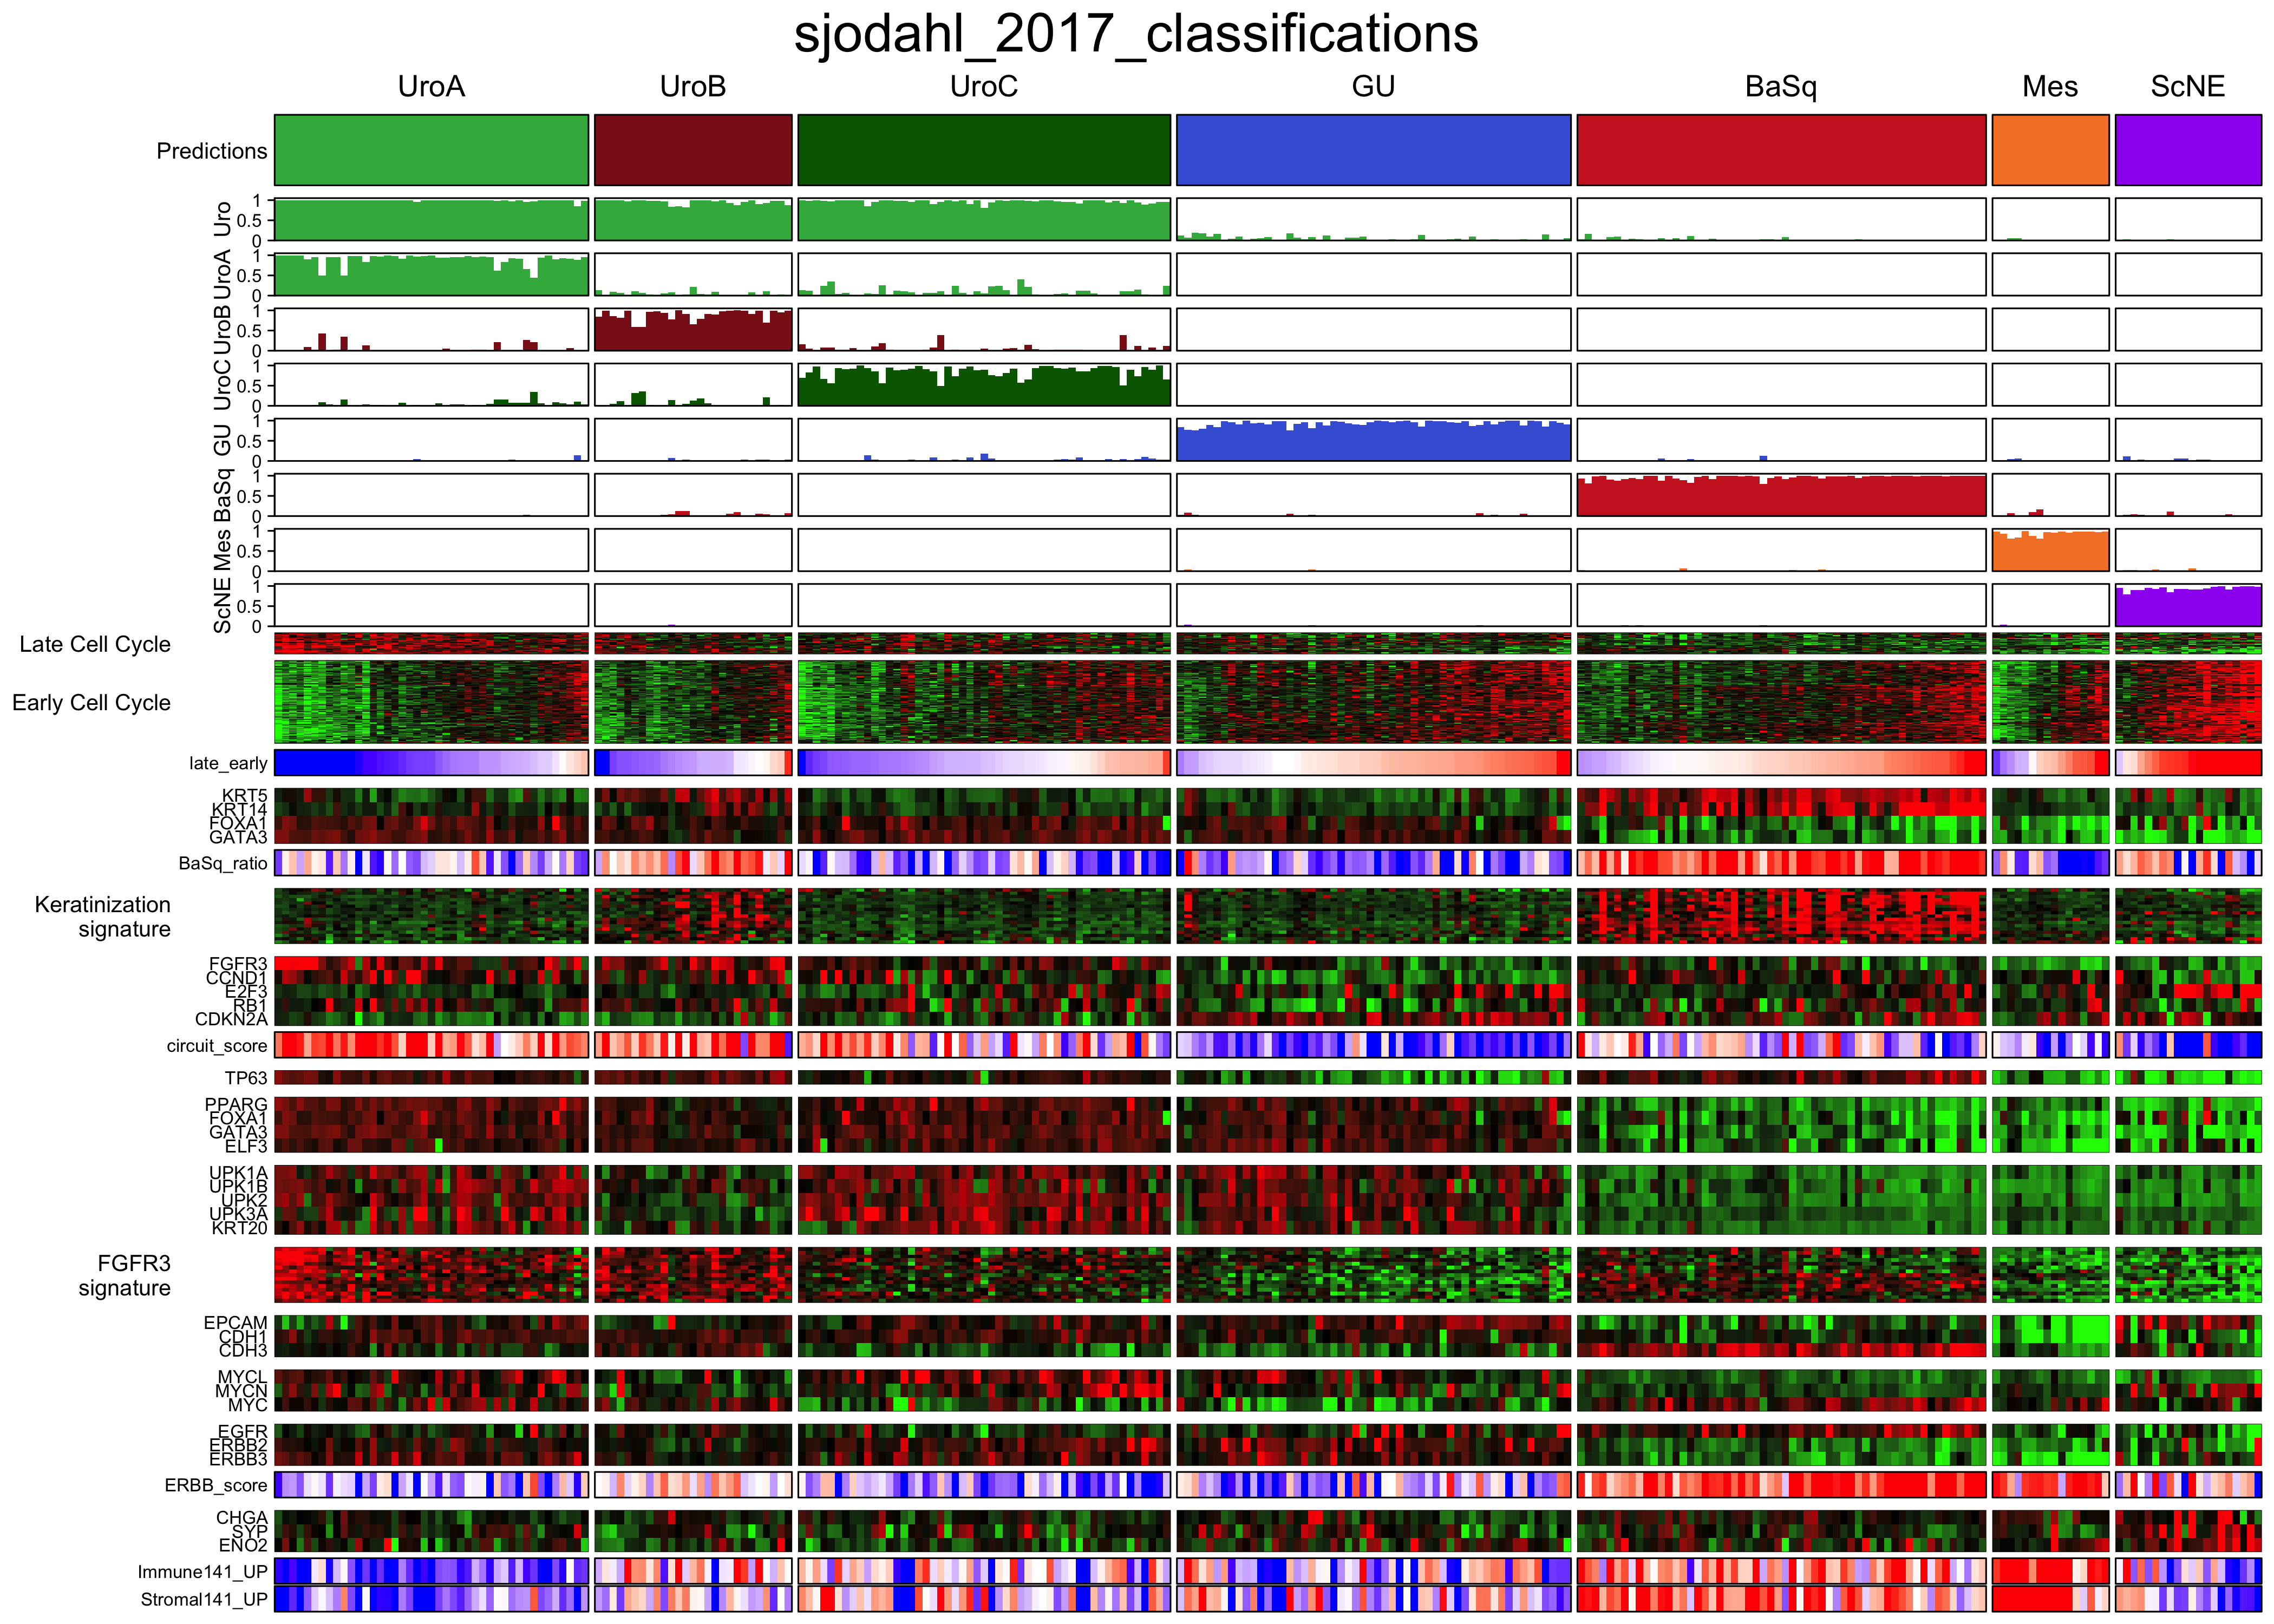
\includegraphics[width=1\linewidth]{../man/figures/sjodahl_2017_classifications_heatmap_scores} \end{center}

\subsubsection{Plot Heatmap Signatures}\label{plot-heatmap-signatures-1}

This functions builds a heatmap for the signature scores (4th element in
the returned list with the classifier function). This allows for a rapid
and comprehenssive overview of how the different signature scores can
relate to the different subtypes. In this example, again, we are using
the prediction calls from the classifier in the example. The function is
called with default paraemters.

\begin{center}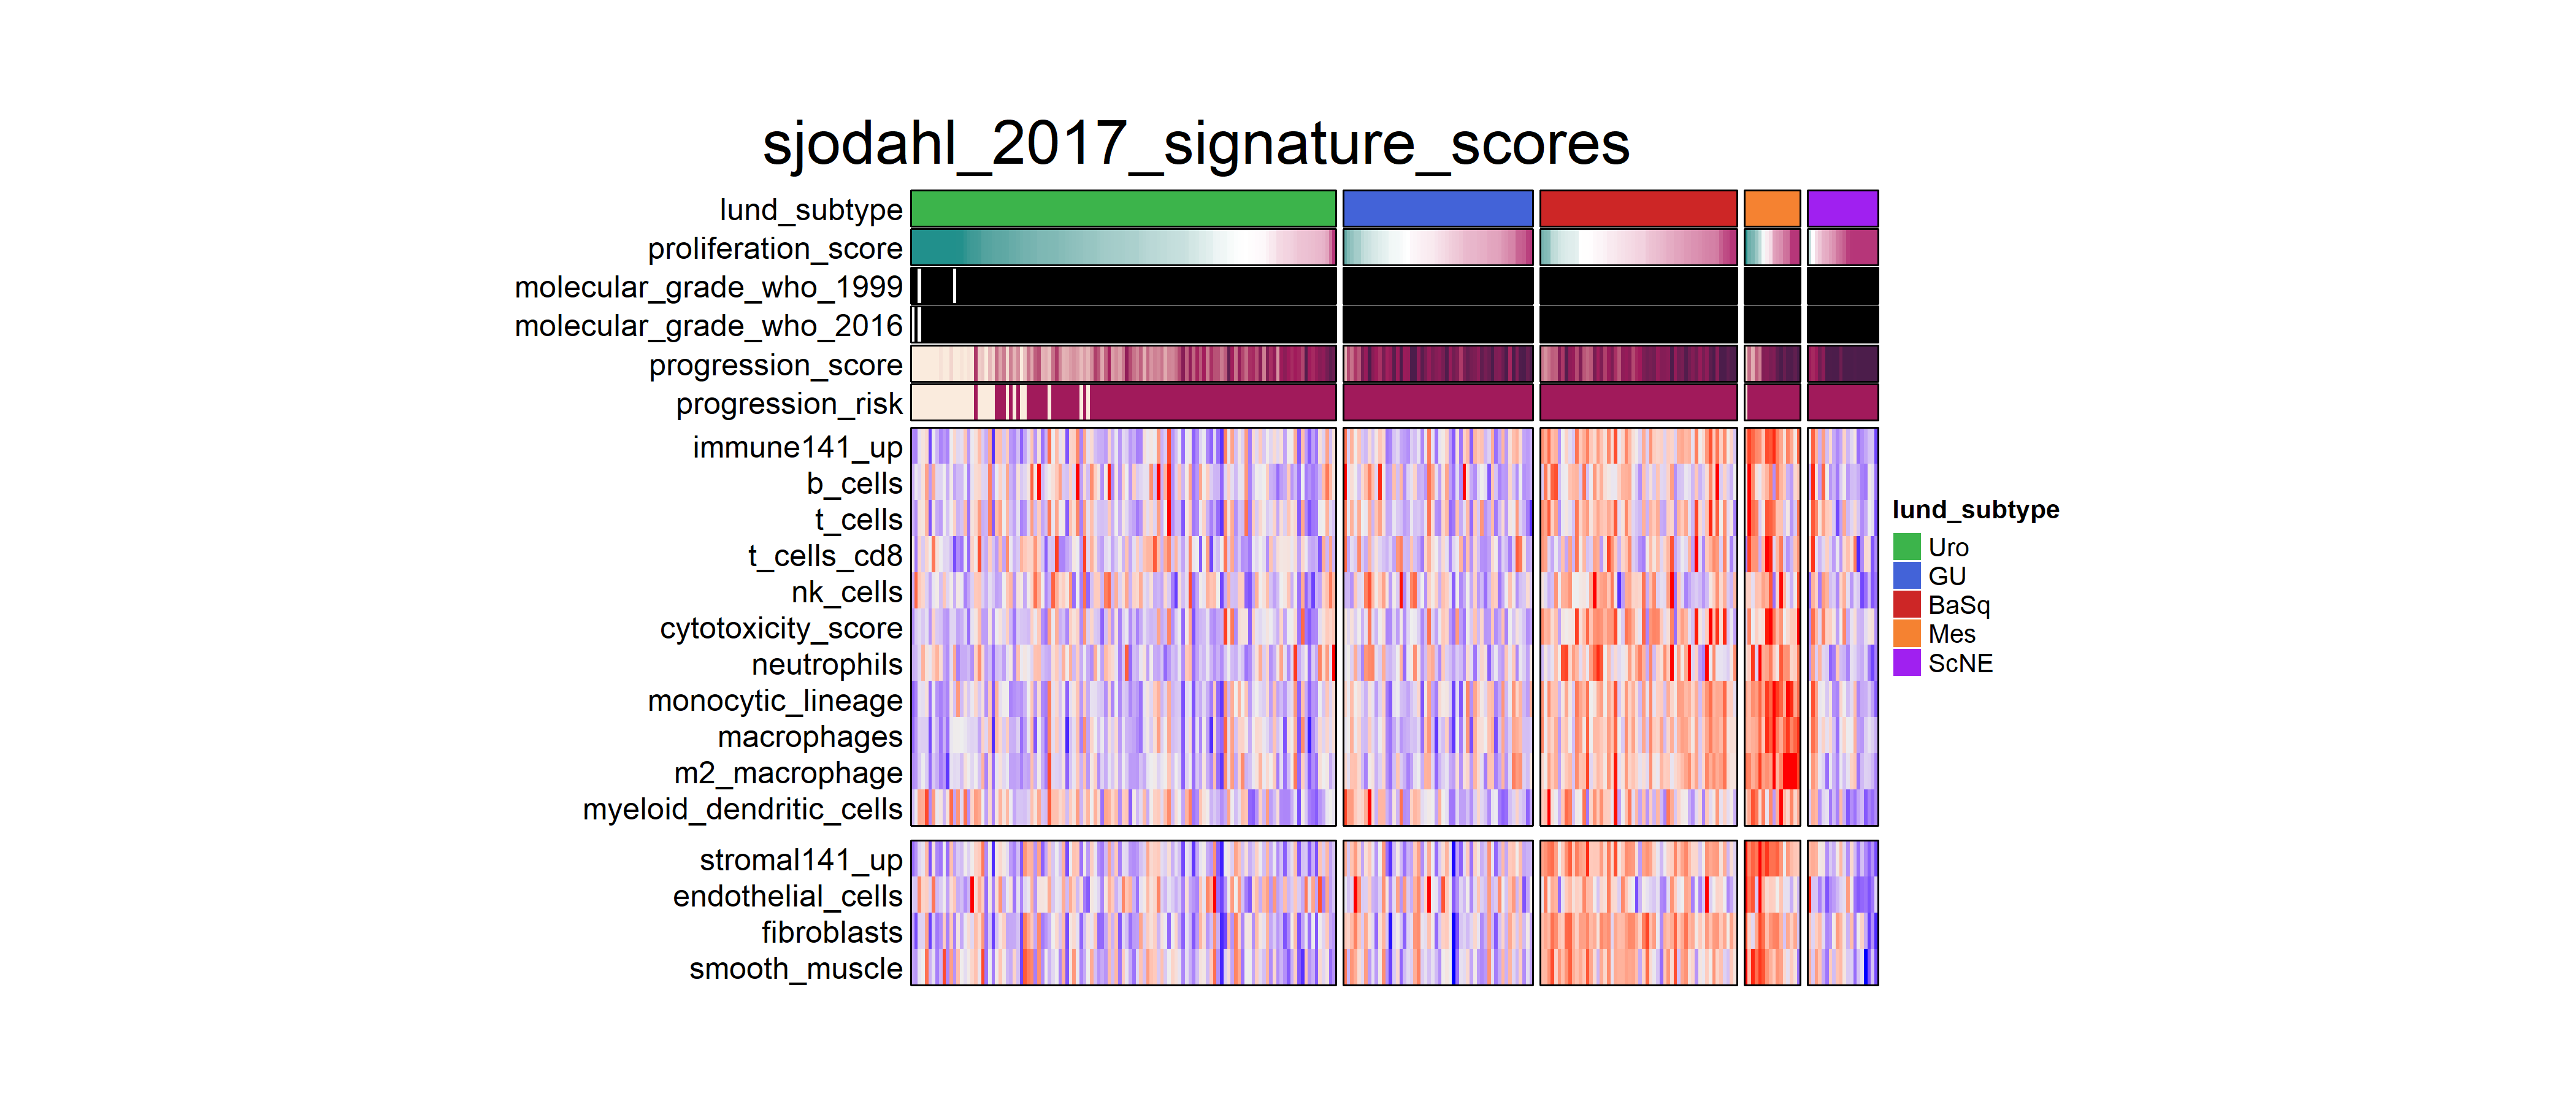
\includegraphics[width=1\linewidth]{../man/figures/sjodahl_2017_signature_scores_heatmap_scores} \end{center}

This function can also be run with \texttt{return\_scores\ =\ TRUE} to
return the plotting data in a tidy format for the user to either run
their own ploting scripts or, aggregating with clinical data, etc. Let's
return this version of the data with the function and see what it looks
like.

\begin{verbatim}
## No output path provided, returning the score data frame in tidy format...
\end{verbatim}

Let's print the column names and type of the returned scores data frame.

\begin{Shaded}
\begin{Highlighting}[]
\FunctionTok{str}\NormalTok{(sjodahl\_scores)}
\end{Highlighting}
\end{Shaded}

\begin{verbatim}
## 'data.frame':    267 obs. of  36 variables:
##  $ proliferation_score               : num  0.731 1.042 0.485 0.66 0.808 ...
##  $ progression_score                 : num  0.768 0.992 0.582 0.78 0.63 ...
##  $ progression_risk                  : Factor w/ 2 levels "HR","LR": 1 1 1 1 1 1 2 1 1 1 ...
##  $ molecular_grade_who_2016_score    : num  0.774 0.746 0.658 0.812 0.781 ...
##  $ molecular_grade_who_2016          : Factor w/ 2 levels "HG","LG": 1 1 1 1 1 1 1 1 1 1 ...
##  $ molecular_grade_who_1999_score    : num  0.807 0.856 0.729 0.865 0.732 ...
##  $ molecular_grade_who_1999          : Factor w/ 2 levels "G1_2","G3": 2 2 2 2 2 2 2 2 2 2 ...
##  $ stromal141_up                     : num  1.88 1.93 1.92 1.88 1.87 ...
##  $ immune141_up                      : num  1.91 2 2.01 1.91 1.94 ...
##  $ b_cells                           : num  1.77 1.79 1.91 1.78 1.77 ...
##  $ b_cells_proportion                : num  0.0737 0.0718 0.0766 0.0735 0.0728 ...
##  $ t_cells                           : num  1.82 1.9 1.97 1.84 1.85 ...
##  $ t_cells_proportion                : num  0.0758 0.0759 0.0787 0.0757 0.0764 ...
##  $ t_cells_cd8                       : num  1.54 1.55 1.7 1.61 1.62 ...
##  $ t_cells_cd8_proportion            : num  0.0638 0.0622 0.0679 0.0663 0.0669 ...
##  $ nk_cells                          : num  1.76 1.8 1.79 1.78 1.79 ...
##  $ nk_cells_proportion               : num  0.0731 0.0721 0.0715 0.0736 0.0739 ...
##  $ cytotoxicity_score                : num  1.81 1.87 1.87 1.83 1.84 ...
##  $ cytotoxicity_score_proportion     : num  0.075 0.075 0.0747 0.0757 0.0758 ...
##  $ neutrophils                       : num  1.79 1.87 1.82 1.8 1.83 ...
##  $ neutrophils_proportion            : num  0.0744 0.0748 0.0729 0.0743 0.0756 ...
##  $ monocytic_lineage                 : num  1.92 2.07 1.98 1.94 1.92 ...
##  $ monocytic_lineage_proportion      : num  0.0798 0.0828 0.0791 0.0801 0.0794 ...
##  $ macrophages                       : num  1.96 2.11 1.99 1.99 1.97 ...
##  $ macrophages_proportion            : num  0.0813 0.0846 0.0797 0.0821 0.0813 ...
##  $ m2_macrophage                     : num  1.87 2.06 1.91 1.87 1.82 ...
##  $ m2_macrophage_proportion          : num  0.0776 0.0824 0.0765 0.0772 0.0752 ...
##  $ myeloid_dendritic_cells           : num  1.74 1.8 1.86 1.76 1.8 ...
##  $ myeloid_dendritic_cells_proportion: num  0.0724 0.0721 0.0742 0.0724 0.0742 ...
##  $ endothelial_cells                 : num  1.85 1.89 1.89 1.86 1.87 ...
##  $ endothelial_cells_proportion      : num  0.0769 0.0755 0.0755 0.0769 0.0772 ...
##  $ fibroblasts                       : num  2.14 2.17 2.16 2.09 2.09 ...
##  $ fibroblasts_proportion            : num  0.0889 0.087 0.0862 0.0864 0.0864 ...
##  $ smooth_muscle                     : num  2.1 2.09 2.16 2.08 2.06 ...
##  $ smooth_muscle_proportion          : num  0.0873 0.0838 0.0864 0.0858 0.0849 ...
##  $ cohort                            : Factor w/ 1 level "sjodahl_2017": 1 1 1 1 1 1 1 1 1 1 ...
\end{verbatim}

The function can also return the data from in xlsx format. To do so, run
the function with \texttt{return\_xlsx\ =\ TRUE}.

\subsubsection{Plot Ranked Score}\label{plot-ranked-score}

This function returns a point plot with ranked scores for a set
variable. It takes a predictions data set together with a score
variable, subtype class and returns a point plot (grob) with ranked
scores along the x axis and scores along the y axis. The returned plot
will also color fill the points based on subtype classification. In this
example, we are plotting proliferation score for all subtypes in the 7
class group.

\begin{center}\includegraphics[width=1\linewidth]{tutorial_files/figure-latex/figure 3-1} \end{center}

\end{document}
